Als Gruppe wollten wir sehr gerne die Oberkante des Basaltgangs mit der Refraktionsseismik detektieren. Von den Betreuern Eva und Fabian wussten wir aber, dass Gruppen in den Vorjahren Schwierigkeiten damit hatten. Wir entschieden uns also, zunächst auf einer anderen Wiese (Messgebiet 2 in Abbildung \ref{fig:MG}) ein langes Profil anzulegen. Erst danach führten wir die Messung beim Basaltgang durch, der sich unter Messgebiet 1 aus Abbildung \ref{fig:MG} befindet, was aus der Magnetik-Kartierung bekannt war. Das Messprotokoll befindet sich in Abbildung \ref{fig:messprotokoll} im Anhang.

\begin{figure}[!ht]
 \centering
 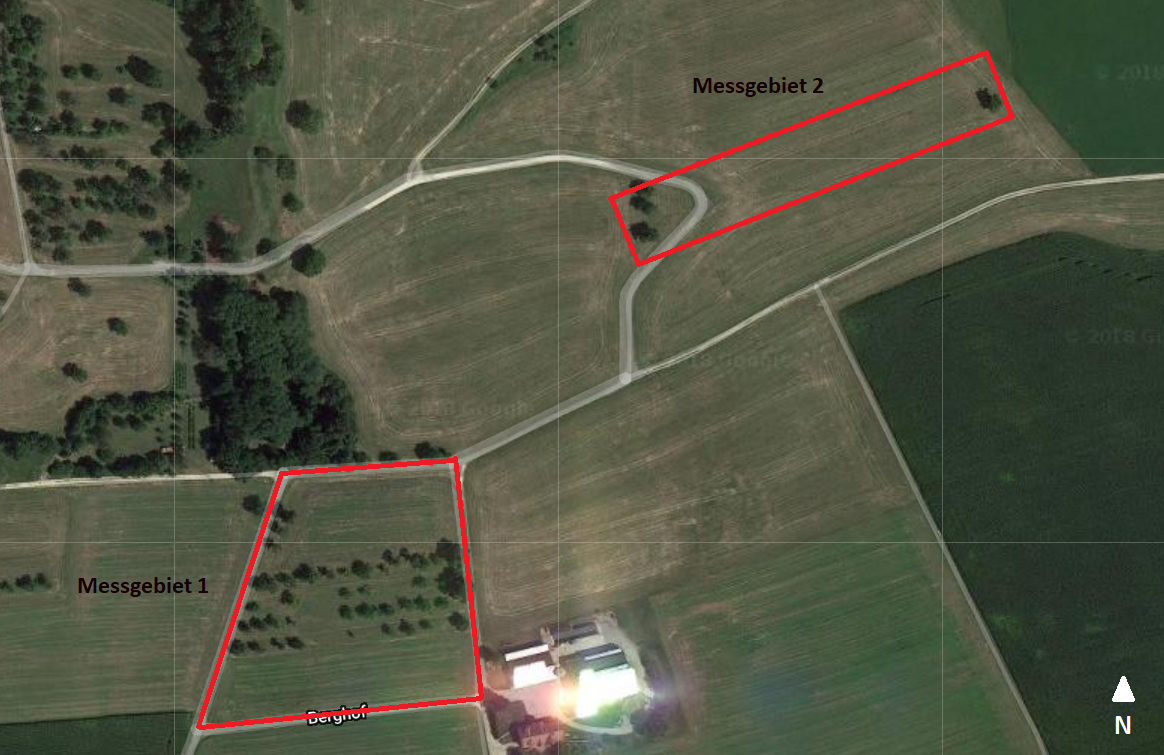
\includegraphics[width=0.8\textwidth]{fig/Messgebiete}
 \caption[Lage der Messgebiete der Seismik-Messungen]{Lage der Messgebiete der Seismik-Messungen. Die Grafik wurde von Rebekka Kirchgässner und Luisa Rank übernommen.}
 \label{fig:MG}
\end{figure}

\section{Profil S11-S12}

Dies ist das Profil im Messgebiet 2. Bei der Refraktionsseismik wird die Annahme getroffen, dass ebene, homogene Schichten im Untergrund vorliegen. Bei geradem Boden ist die Wahrscheinlichkeit größer, dass dies näherungsweise der Fall ist. Wir versuchten also eine möglichst flache Stelle zu finden, was sich aufgrund der ausgeprägten Topographie jedoch als sehr schwierig herausstellte. Man konnte wegen eines Hügels vom einen Ende des Profils das andere Ende nicht sehen. Es wurden 72 Geophone verwendet. In Abbildung \ref{fig:Lea1} ist die Lage der Geophone eingezeichnet. Da für S.I.S.Sy ein Loch gebohrt werden musste, ist dieses Profil ein Meter länger als das Hammerschlag-Profil.

\begin{figure}[!ht]
 \centering
 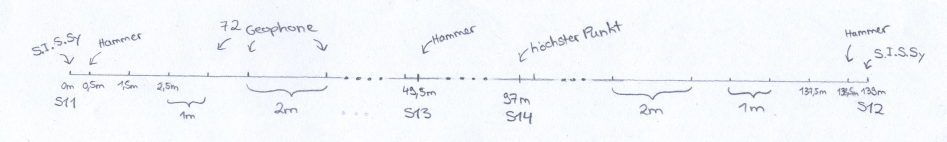
\includegraphics[width=\textwidth]{fig/Skizze1}
 \caption{Lage der 72 Geophone bei Profil S11-S12}
 \label{fig:Lea1}
\end{figure}

\subsection{Hammerschlag}

Von den Betreuern wurde uns empfohlen, beim Hammerschlag einen Hin-, Rück- und Mittelschuss durchzuführen, weil die Gesamtlänge von 138\,m durch Hammerschläge vermutlich nicht erreicht werden kann. Außerdem stapelten wir bei der Messung mit Hammerschlag jeweils 5 Messungen, um ein besseres Signal-Rausch-Verhältnis zu erreichen. Der Punkt des Mittelschuss wurde S13 genannt und befindet sich 49\,m vom Punkt des Hinschusses S11 entfernt, wie in Abbildung \ref{fig:Lea1} eingezeichnet.

\subsection{Verpuffungsquelle S.I.S.Sy}

Bei der Messung mit der Verpuffungsquelle S.I.S.Sy als  Signalquelle musste nur ein Hin- und ein Rückschuss durchgeführt werden, da sie eine höhere Energie als ein Hammerschlag aufweist. Die Löcher wurden genau an den Ende des Profils gebohrt, was zu einer Gesamtlänge dieser Auslage von 139\,m ergab. Beim Bohren ergab sich die Schwierigkeit, dass wir das erste Loch mit einem Knick bohrten und so S.I.S.Sy nicht hineinpasste. Außerdem stießen wir in einer Tiefe von ca. 60\,cm auf eine Schicht mit sehr vielen Steinen.

\section{Profile beim Basaltgang}

Nun untersuchten wir noch den Basaltgang mit der Refraktionsseismik. Dazu legten wir ein Profil über dem Basaltgang und eines weit neben ihm an. Das zweite Profil soll zum Vergleich dienen, um zu sehen, ob der Gang mit der Seismik überhaupt detektiert werden kann. Bei beiden Profilen wurden 24 Geophone auf einer Länge von 42\,m verwendet (Siehe Abbildung \ref{fig:Lea2}). Wegen der geringen Länge wurden nur Hin- und Rückschüsse mit Hammerschlag durchgeführt. Es wurden wieder 5 Seismogramme gestapelt.

\begin{figure}[!ht]
 \centering
 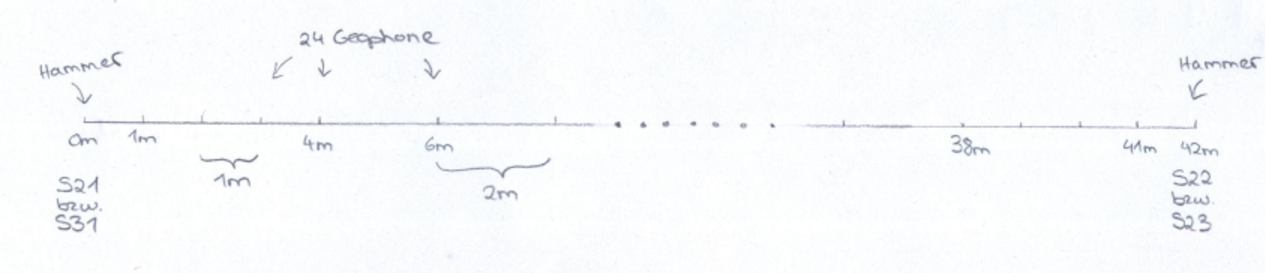
\includegraphics[width=\textwidth]{fig/Skizze2}
 \caption{Lage der 24 Geophone bei Profil S21-S22 und S31-S32}
 \label{fig:Lea2}
\end{figure}

\subsection{Profil S21-S22}

Dieses Profil legten wir so an, dass es möglichst parallel zum und genau über dem Basaltgang war. Dazu nutzten wir unser Wissen über die Lage des Basaltgangs aus der Magnetik-Kartierung vom Vortag.

\subsection{Profil S31-S32}

Per Augenmaß parallel zu Profil S21-S22 legten wir dieses Profil an, das möglichst weit weg vom Basaltgang sein sollte, um ausschließen zu können, dass er noch einen Einfluss auf die Messergebisse hat. Die Lage beider Profile ist in Abbildung \ref{fig:kleineProfile} eingezeichnet.

\begin{figure}[!ht]
 \centering
 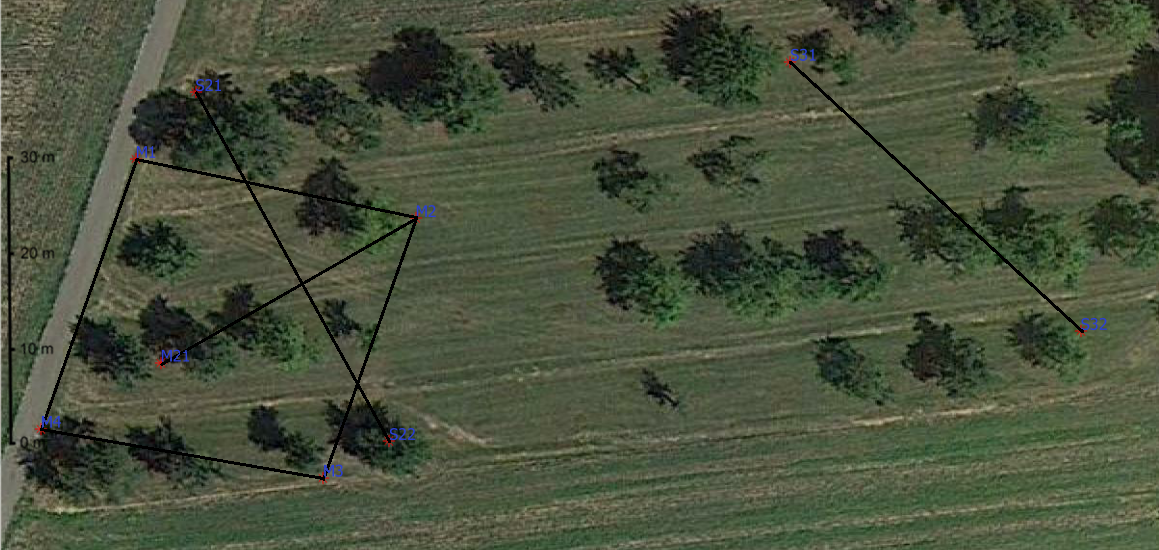
\includegraphics[width=\textwidth]{fig/Seismik_klein_verbund}
 \caption[Lage der Profile S21-S22 und S31-S32]{Lage der Profile S21-S22 und S31-S32. Die ungefähr in Nord-Süd-Richtung verlaufenden Profile sind die Profile S21-S22 und S31-S32. Auf dem Quadrat wurde die Magnetik-Kartierung durchgeführt. Die Grafik wurde von Katharina Adrion und Niels Gieseler übernommen.}
 \label{fig:kleineProfile}
\end{figure}

% \begin{figure}[!ht]
%  \centering
%  \includegraphics[width=\textwidth]{fig/}
%  \caption{}
%  \label{fig:}
% \end{figure}